% =====================================================================
%  Capítulo 12. Volatilidad multivariada y correlaciones dinámicas
% =====================================================================
\chapter[Correlaciones dinámicas]{Volatilidad multivariada: EWMA, correlación condicional constante y DCC}\label{cap:dcc}

\section*{Objetivos de aprendizaje}
Al terminar este capítulo, el lector podrá:
\begin{enumerate}[label=\arabic*.,leftmargin=*]
  \item Explicar por qué modelar matrices de covarianza condicionales es difícil y cómo lo resuelven los modelos
        EWMA, CCC y DCC.
  \item Demostrar que la verosimilitud del DCC se separa en una parte de volatilidad y otra de correlación, y
        estimar el modelo en dos etapas.
  \item Usar las covarianzas condicionales para construir carteras de mínima varianza y evaluarlas fuera de
        muestra.
  \item Distinguir el aumento de correlación por contagio del que produce mecánicamente un aumento de
        volatilidad (Forbes y Rigobon).
\end{enumerate}

\section*{Motivación}
La diversificación descansa en una cifra: la correlación entre los activos. Si es baja, combinar activos reduce
el riesgo; si sube justo cuando los mercados caen, la protección desaparece cuando más se necesita. Los
Capítulos~\ref{cap:garch} y~\ref{cap:asimetria} mostraron que las volatilidades cambian en el tiempo; este
capítulo muestra que las correlaciones también. La correlación entre el petróleo y las acciones de EE.\,UU.,
por ejemplo, era casi nula antes de 2008 y luego se volvió claramente positiva. Gestionar carteras, calcular
el riesgo de una posición cubierta o medir el contagio entre mercados exige modelar la matriz de covarianzas
completa.

\paragraph{Datos del capítulo.} Rendimientos logarítmicos diarios del S\&P 500 y del Nasdaq Composite (Yahoo
Finance) y del Brent (EIA), en los 4\,615 días en que los tres cotizaron entre enero de 1999 y diciembre de 2018.
Cuando un mercado cierra y otro no, el rendimiento del día siguiente abarca dos días; con datos diarios de
mercados de distintos países esa falta de sincronía es inevitable y tiende a reducir las correlaciones medidas.

% ---------------------------------------------------------------------
\section{La matriz de covarianzas condicional}
% ---------------------------------------------------------------------

Sea $\boldsymbol\varepsilon_t=\mathbf r_t-\boldsymbol\mu$ el vector de $K$ innovaciones, con
\[
  \E[\boldsymbol\varepsilon_t\mid\mathcal F_{t-1}]=\mathbf 0,\qquad
  \Var(\boldsymbol\varepsilon_t\mid\mathcal F_{t-1})=H_t .
\]
Un modelo para $H_t$ debe cumplir dos requisitos: que $H_t$ sea definida positiva en todo momento (de lo
contrario alguna cartera tendría varianza negativa) y que el número de parámetros no explote con $K$. La
generalización directa del GARCH, en la que cada elemento de $H_t$ depende de todos los productos
$\varepsilon_{i,t-1}\varepsilon_{j,t-1}$, tiene del orden de $K^4$ parámetros: con $K=10$, más de 6\,000. Los
modelos de este capítulo resuelven el problema separando volatilidades y correlaciones.

\subsection{EWMA multivariado}

La extensión de RiskMetrics aplica la misma media móvil exponencial a cada varianza y covarianza:
\[
  H_t=\lambda H_{t-1}+(1-\lambda)\,\boldsymbol\varepsilon_{t-1}\boldsymbol\varepsilon_{t-1}',\qquad\lambda=0{,}94 .
\]
Como $\boldsymbol\varepsilon\boldsymbol\varepsilon'$ es semidefinida positiva, $H_t$ es definida positiva si
$H_{t-1}$ lo es. No requiere estimación, pero impone la misma persistencia a todas las varianzas y covarianzas,
y no tiene nivel de largo plazo (es un IGARCH).

\subsection{Correlación condicional constante (CCC)}

Bollerslev (1990) propuso descomponer
\[
  H_t=D_tRD_t,\qquad D_t=\operatorname{diag}(\sigma_{1t},\dots,\sigma_{Kt}),
\]
donde cada $\sigma_{it}^2$ sigue un GARCH univariado y $R$ es una matriz de correlaciones constante. La covarianza
$h_{ij,t}=\rho_{ij}\sigma_{it}\sigma_{jt}$ cambia solo porque cambian las volatilidades.

\subsection{Correlación condicional dinámica (DCC)}

\begin{definicion}[DCC(1,1); Engle, 2002]
Sea $\mathbf z_t=D_t^{-1}\boldsymbol\varepsilon_t$ el vector de residuos estandarizados de los GARCH univariados
y $\bar Q=\frac1T\sum_t\mathbf z_t\mathbf z_t'$. Con $a,b\ge0$ y $a+b<1$,
\begin{align*}
  Q_t &= (1-a-b)\,\bar Q+a\,\mathbf z_{t-1}\mathbf z_{t-1}'+b\,Q_{t-1},\\
  R_t &= \operatorname{diag}(Q_t)^{-1/2}\,Q_t\,\operatorname{diag}(Q_t)^{-1/2},\\
  H_t &= D_tR_tD_t .
\end{align*}
\end{definicion}

La matriz $Q_t$ es un GARCH(1,1) escalar para los productos de residuos estandarizados, con nivel de largo plazo
$\bar Q$ (\emph{correlation targeting}). Su diagonal no es exactamente uno, así que se reescala para obtener una
matriz de correlaciones. Con solo dos parámetros, sea cual sea $K$, el modelo permite que todas las correlaciones
cambien, aunque con la misma dinámica.

\begin{proposicion}[$R_t$ es una matriz de correlaciones definida positiva]\label{prop:dccpd}
Si $\bar Q$ y $Q_0$ son definidas positivas, $a,b\ge0$ y $a+b<1$, entonces $Q_t$ es definida positiva para todo
$t$, y $R_t$ es una matriz de correlaciones definida positiva.
\end{proposicion}

\begin{proof}
Por inducción. Supongamos $Q_{t-1}$ definida positiva. Para todo $\mathbf x\ne\mathbf 0$:
\begin{align*}
  \mathbf x'Q_t\mathbf x &= (1-a-b)\,\mathbf x'\bar Q\mathbf x+a\,\mathbf x'\mathbf z_{t-1}\mathbf z_{t-1}'\mathbf x+b\,\mathbf x'Q_{t-1}\mathbf x\\
                         &= (1-a-b)\,\mathbf x'\bar Q\mathbf x+a\,(\mathbf z_{t-1}'\mathbf x)^2+b\,\mathbf x'Q_{t-1}\mathbf x .
\end{align*}
El primer término es estrictamente positivo porque $1-a-b>0$ y $\bar Q$ es definida positiva; los otros dos son
no negativos. Luego $\mathbf x'Q_t\mathbf x>0$. Para $R_t$, sea $S=\operatorname{diag}(Q_t)^{-1/2}$, que es diagonal
con elementos positivos, y $\mathbf y=S\mathbf x\ne\mathbf 0$:
\begin{align*}
  \mathbf x'R_t\mathbf x &= \mathbf x'SQ_tS\mathbf x\\
                         &= (S\mathbf x)'Q_t(S\mathbf x)\\
                         &= \mathbf y'Q_t\mathbf y>0 .
\end{align*}
Su diagonal es $[R_t]_{ii}=q_{ii,t}/\sqrt{q_{ii,t}q_{ii,t}}=1$. Una matriz simétrica definida positiva con unos
en la diagonal es una matriz de correlaciones: por la desigualdad de Cauchy-Schwarz, sus elementos fuera de la
diagonal están entre $-1$ y $1$.
\end{proof}

\paragraph{Curva de impacto de la correlación.} ¿Cómo responde la correlación a las noticias? Si hoy dos activos
reciben choques del mismo signo, $z_{1}z_{2}>0$ y $q_{12}$ sube; si son de signo opuesto, baja. La
Figura~\ref{fig:dccteoria} (derecha) lo muestra con $a=0{,}05$, $b=0{,}93$ y una correlación de partida de
$0{,}3$: dos choques de $+2$ desviaciones estándar la elevan a $0{,}42$; choques de $+2$ y $-2$ la reducen a $0{,}07$.
Los contornos tienen forma de silla de montar: la correlación sube en los cuadrantes primero y tercero, y baja en
los otros dos.

% ---------------------------------------------------------------------
\section{Estimación en dos etapas}
% ---------------------------------------------------------------------

\begin{proposicion}[Separación de la verosimilitud]\label{prop:dccll}
Con innovaciones normales, la log-verosimilitud de $\boldsymbol\varepsilon_t\mid\mathcal F_{t-1}\sim N(\mathbf 0,H_t)$
con $H_t=D_tR_tD_t$ se separa en
\begin{align*}
  \ell &= \ell_V+\ell_C,\\
  \ell_V &= -\frac12\sum_{t}\sum_{i=1}^{K}\Bigl[\ln(2\pi)+\ln\sigma_{it}^2+\frac{\varepsilon_{it}^2}{\sigma_{it}^2}\Bigr],\\
  \ell_C &= -\frac12\sum_{t}\Bigl[\ln|R_t|+\mathbf z_t'R_t^{-1}\mathbf z_t-\mathbf z_t'\mathbf z_t\Bigr].
\end{align*}
$\ell_V$ es la suma de las verosimilitudes de $K$ GARCH univariados y solo $\ell_C$ depende de $(a,b)$.
\end{proposicion}

\begin{proof}
La densidad normal multivariada da
\begin{align*}
  \ell_t &= -\frac12\Bigl[K\ln(2\pi)+\ln|H_t|+\boldsymbol\varepsilon_t'H_t^{-1}\boldsymbol\varepsilon_t\Bigr].
\end{align*}
El determinante de un producto es el producto de los determinantes, y $|D_t|=\prod_i\sigma_{it}$:
\begin{align*}
  \ln|H_t| &= \ln|D_t|+\ln|R_t|+\ln|D_t|\\
           &= \sum_{i=1}^{K}\ln\sigma_{it}^2+\ln|R_t| .
\end{align*}
Para la forma cuadrática, con $H_t^{-1}=D_t^{-1}R_t^{-1}D_t^{-1}$ y $\mathbf z_t=D_t^{-1}\boldsymbol\varepsilon_t$:
\begin{align*}
  \boldsymbol\varepsilon_t'H_t^{-1}\boldsymbol\varepsilon_t &= (D_t^{-1}\boldsymbol\varepsilon_t)'R_t^{-1}(D_t^{-1}\boldsymbol\varepsilon_t)\\
                                                           &= \mathbf z_t'R_t^{-1}\mathbf z_t .
\end{align*}
Sumamos y restamos $\mathbf z_t'\mathbf z_t=\sum_i\varepsilon_{it}^2/\sigma_{it}^2$:
\begin{align*}
  \ell_t &= -\frac12\Bigl[K\ln(2\pi)+\sum_i\ln\sigma_{it}^2+\ln|R_t|+\mathbf z_t'R_t^{-1}\mathbf z_t\Bigr]\\
         &= -\frac12\Bigl[K\ln(2\pi)+\sum_i\ln\sigma_{it}^2+\mathbf z_t'\mathbf z_t\Bigr]
            -\frac12\Bigl[\ln|R_t|+\mathbf z_t'R_t^{-1}\mathbf z_t-\mathbf z_t'\mathbf z_t\Bigr]\\
         &= -\frac12\sum_{i=1}^{K}\Bigl[\ln(2\pi)+\ln\sigma_{it}^2+\frac{\varepsilon_{it}^2}{\sigma_{it}^2}\Bigr]
            -\frac12\Bigl[\ln|R_t|+\mathbf z_t'R_t^{-1}\mathbf z_t-\mathbf z_t'\mathbf z_t\Bigr].
\end{align*}
Sumando sobre $t$ se obtiene $\ell=\ell_V+\ell_C$. Restar $\mathbf z_t'\mathbf z_t$ en $\ell_C$ no cambia su
máximo respecto de $(a,b)$; solo hace que $\ell_C=0$ cuando $R_t=I$.
\end{proof}

La proposición justifica el procedimiento de Engle (2002): (1) estimar un GARCH univariado para cada serie y
calcular $\mathbf z_t$; (2) maximizar $\ell_C$ respecto de $(a,b)$ con $\bar Q$ fijo en su valor muestral. El
estimador es consistente, aunque menos eficiente que la máxima verosimilitud conjunta; los errores estándar de
la segunda etapa, si se calculan con la hessiana de $\ell_C$, ignoran la incertidumbre de la primera y tienden a
ser optimistas. El CCC es el caso $a=b=0$ con $R_t=R$; la razón de verosimilitudes $2(\ell_C^{\text{DCC}}-\ell_C^{\text{CCC}})$
mide la ganancia de dejar que la correlación cambie. Su distribución no es exactamente $\chi^2_2$, porque bajo
$a=0$ el parámetro $b$ no está identificado, pero una cifra muy grande deja poca duda.

% ---------------------------------------------------------------------
\section{Aplicaciones}
% ---------------------------------------------------------------------

\subsection{Cartera de mínima varianza}

\begin{proposicion}[Cartera de mínima varianza]\label{prop:minvar}
Con matriz de covarianzas $H$ definida positiva, los pesos que minimizan la varianza $\mathbf w'H\mathbf w$ sujeto a
$\mathbf w'\boldsymbol\iota=1$ (con $\boldsymbol\iota$ un vector de unos) son
\[
  \mathbf w^*=\frac{H^{-1}\boldsymbol\iota}{\boldsymbol\iota'H^{-1}\boldsymbol\iota},\qquad
  \mathbf w^{*\prime}H\mathbf w^*=\frac{1}{\boldsymbol\iota'H^{-1}\boldsymbol\iota}.
\]
\end{proposicion}

\begin{proof}
El lagrangiano es $\mathcal L=\mathbf w'H\mathbf w-\lambda(\mathbf w'\boldsymbol\iota-1)$. La condición de
primer orden da
\begin{align*}
  \frac{\partial\mathcal L}{\partial\mathbf w} &= 2H\mathbf w-\lambda\boldsymbol\iota=\mathbf 0,\\
  \mathbf w &= \frac\lambda2\,H^{-1}\boldsymbol\iota .
\end{align*}
La restricción fija $\lambda$:
\begin{align*}
  \boldsymbol\iota'\mathbf w &= \frac\lambda2\,\boldsymbol\iota'H^{-1}\boldsymbol\iota=1,\\
  \frac\lambda2 &= \frac{1}{\boldsymbol\iota'H^{-1}\boldsymbol\iota}.
\end{align*}
Sustituyendo se obtiene $\mathbf w^*$. Su varianza es
\begin{align*}
  \mathbf w^{*\prime}H\mathbf w^* &= \frac{\boldsymbol\iota'H^{-1}HH^{-1}\boldsymbol\iota}{(\boldsymbol\iota'H^{-1}\boldsymbol\iota)^2}\\
                                  &= \frac{\boldsymbol\iota'H^{-1}\boldsymbol\iota}{(\boldsymbol\iota'H^{-1}\boldsymbol\iota)^2}\\
                                  &= \frac{1}{\boldsymbol\iota'H^{-1}\boldsymbol\iota}.
\end{align*}
Es un mínimo porque $H$ es definida positiva.
\end{proof}

Con $H_t$ condicional, los pesos cambian cada día. La comparación de modelos de covarianza mediante la varianza
realizada de las carteras que generan es un criterio económico, no solo estadístico (Engle y Colacito, 2006): el
mejor modelo es el que produce la cartera menos riesgosa fuera de la muestra.

\subsection{Contagio y el sesgo de la correlación condicionada}

Que la correlación medida suba en una crisis no prueba que haya contagio. Forbes y Rigobon (2002) mostraron que
la correlación aumenta mecánicamente cuando aumenta la volatilidad del mercado de origen, aunque la relación
entre los mercados no cambie.

\begin{proposicion}[Sesgo de Forbes y Rigobon]\label{prop:forbes}
Sea $y=\beta x+e$ con $e$ no correlacionado con $x$ y $\beta$ y $\Var(e)$ iguales en calma y en crisis. Si en la
crisis la varianza de $x$ aumenta en un factor $1+\delta$, la correlación pasa de $\rho$ a
\[
  \rho_c=\rho\,\sqrt{\frac{1+\delta}{1+\delta\rho^2}} .
\]
Por tanto, la correlación en la crisis corregida por el sesgo es $\rho^*=\rho_c\big/\sqrt{1+\delta(1-\rho_c^2)}$.
\end{proposicion}

\begin{proof}
En calma, con $\sigma_x^2=\Var(x)$ y $\sigma_e^2=\Var(e)$:
\begin{align*}
  \rho^2 &= \frac{\Cov(x,y)^2}{\Var(x)\Var(y)}\\
         &= \frac{\beta^2\sigma_x^4}{\sigma_x^2(\beta^2\sigma_x^2+\sigma_e^2)}\\
         &= \frac{\beta^2\sigma_x^2}{\beta^2\sigma_x^2+\sigma_e^2}.
\end{align*}
Despejamos $\sigma_e^2$:
\begin{align*}
  \sigma_e^2 &= \beta^2\sigma_x^2\,\frac{1-\rho^2}{\rho^2}.
\end{align*}
En la crisis, $\sigma_x^2$ se convierte en $(1+\delta)\sigma_x^2$ y $\sigma_e^2$ no cambia:
\begin{align*}
  \rho_c^2 &= \frac{\beta^2(1+\delta)\sigma_x^2}{\beta^2(1+\delta)\sigma_x^2+\sigma_e^2}\\
           &= \frac{(1+\delta)}{(1+\delta)+(1-\rho^2)/\rho^2}\\
           &= \frac{(1+\delta)\rho^2}{(1+\delta)\rho^2+1-\rho^2}\\
           &= \frac{(1+\delta)\rho^2}{1+\delta\rho^2}.
\end{align*}
Tomando raíz (con el signo de $\beta$) se obtiene $\rho_c$. Para invertir la relación, despejamos $\rho^2$ de la
última igualdad:
\begin{align*}
  \rho_c^2(1+\delta\rho^2) &= (1+\delta)\rho^2,\\
  \rho_c^2 &= \rho^2\bigl[(1+\delta)-\delta\rho_c^2\bigr],\\
  \rho^2 &= \frac{\rho_c^2}{1+\delta(1-\rho_c^2)}. && \qedhere
\end{align*}
\end{proof}

La Figura~\ref{fig:dccteoria} (izquierda) muestra la magnitud del sesgo: si la varianza del mercado de origen se
cuadruplica ($\delta=3$), una correlación de $0{,}3$ se mide como
\begin{align*}
  \rho_c &= 0{,}3\sqrt{\frac{1+3}{1+3(0{,}09)}}\\
         &= 0{,}3\times\frac{2}{\sqrt{1{,}27}}\\
         &= 0{,}532,
\end{align*}
sin que haya cambiado nada en la relación entre los mercados. La corrección supone que todo el aumento de
volatilidad nace en $x$ y que no hay variables omitidas; si ambos mercados reciben a la vez un choque común,
la corrección es excesiva.

\begin{figure}[ht]
\centering
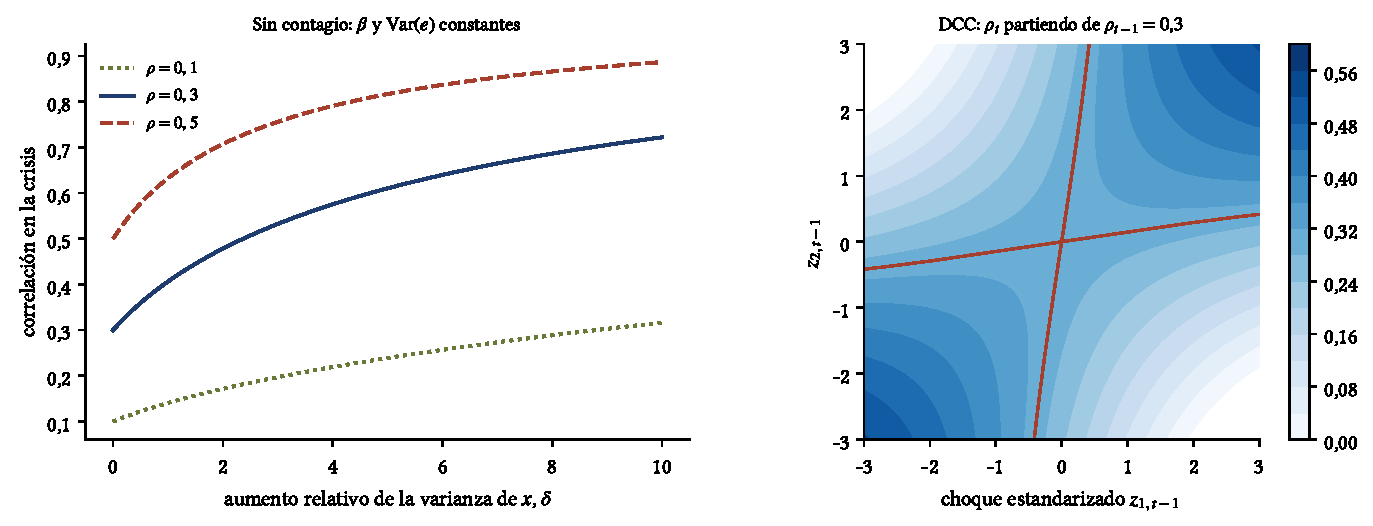
\includegraphics[width=\linewidth]{graficos/cap12_fig_teoria.pdf}
\caption{Izquierda: correlación medida en un período en que la varianza del mercado de origen aumenta un factor
$1+\delta$, sin contagio (Proposición~\ref{prop:forbes}). Derecha: correlación de mañana en un DCC con
$a=0{,}05$ y $b=0{,}93$ según los choques estandarizados de hoy; la línea roja marca los choques que la dejan en
$0{,}3$.}
\label{fig:dccteoria}
\end{figure}

% ---------------------------------------------------------------------
\section{Ejercicios resueltos}
% ---------------------------------------------------------------------

\begin{ejresuelto}{Correlaciones que cambian}\label{ej:corrmov}
\enunciado Calcule las correlaciones diarias entre el S\&P 500, el Nasdaq y el Brent en toda la muestra y por
subperíodos, y las correlaciones con una ventana móvil de 250 días y con EWMA ($\lambda=0{,}94$).

\solucion
\paso{Paso 1. Correlaciones incondicionales.} En toda la muestra, la correlación S\&P--Nasdaq es $0{,}885$ y la
S\&P--Brent, $0{,}139$. Pero por subperíodos:
\begin{center}\small
\begin{tabular}{@{}lrr@{}}
\toprule
Par & 1999--2007 & 2009--2018 \\
\midrule
S\&P--Brent  & 0,006 & 0,299 \\
S\&P--Nasdaq & 0,852 & 0,954 \\
\bottomrule
\end{tabular}
\end{center}
La correlación entre el petróleo y las acciones pasó de cero a $0{,}30$ después de la crisis financiera.

\paso{Paso 2. Correlaciones móviles.} Con EWMA, la correlación S\&P--Brent va de $-0{,}64$ (diciembre de 2004) a
$0{,}74$ (junio de 2012); con la ventana de 250 días, de $-0{,}25$ a $0{,}54$ (Figura~\ref{fig:corrmov}). La EWMA es
mucho más ruidosa: con $\lambda=0{,}94$ su ``memoria'' efectiva es de unos $1/(1-\lambda)\approx17$ días. La ventana
móvil es más suave, pero reacciona tarde y cambia bruscamente cuando una observación extrema sale de la ventana.

\codigoweb{cap12_ej01}
\salidaR{cap12_ej01_R.txt}
\lectura{cap12_ej01}

\RvsPy Las covarianzas EWMA se guardan en un arreglo tridimensional $T\times K\times K$: \texttt{array(0, c(T, K,
K))} en R y \texttt{np.empty((T, K, K))} en Python; \texttt{tcrossprod(e)} de R y \texttt{np.outer(e, e)} calculan
el producto $\boldsymbol\varepsilon\boldsymbol\varepsilon'$. Las funciones del capítulo reutilizan
\texttt{garch\_fit} del Capítulo~\ref{cap:garch} para la primera etapa.

\begin{figure}[ht]
\centering
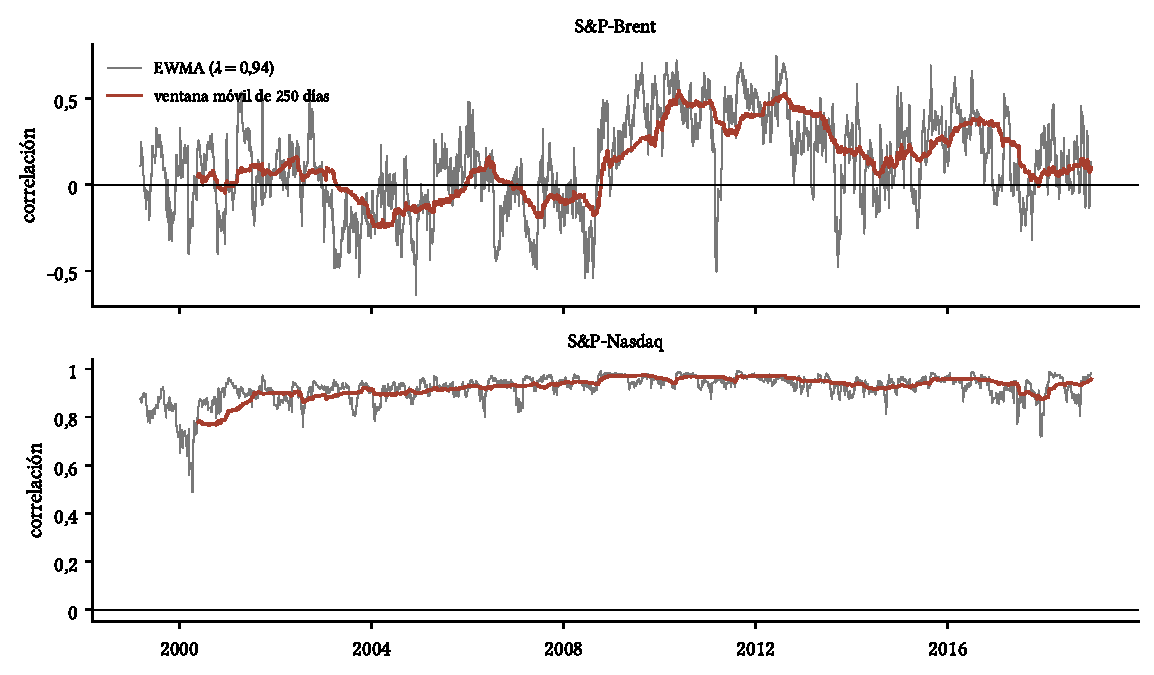
\includegraphics[width=0.92\linewidth]{graficos/cap12_ej01_correlaciones.pdf}
\caption{Correlación diaria S\&P--Brent y S\&P--Nasdaq con EWMA y con ventana móvil de 250 días.}
\label{fig:corrmov}
\end{figure}

\begin{conclusion}
Una sola correlación para veinte años oculta dos regímenes muy distintos. La EWMA y la ventana móvil detectan los
cambios, pero la primera es muy ruidosa y la segunda reacciona con retraso; el DCC busca un punto intermedio
estimado con los datos.
\end{conclusion}
\end{ejresuelto}

\begin{ejresuelto}{DCC para el S\&P 500 y el Brent}\label{ej:dcc2}
\enunciado Estime un DCC(1,1) en dos etapas para el S\&P 500 y el Brent, compárelo con el CCC y describa la
evolución de la correlación.

\solucion
\paso{Paso 1. Primera etapa.} GARCH(1,1) normales: para el S\&P 500, $\hat\alpha=0{,}1024$ y $\hat\beta=0{,}8865$;
para el Brent, $\hat\alpha=0{,}0468$ y $\hat\beta=0{,}9524$ (en esta muestra, que termina en 2018).

\paso{Paso 2. Segunda etapa.}
\begin{align*}
  \hat a &= 0{,}0130\quad(0{,}0027),\\
  \hat b &= 0{,}9844\quad(0{,}0035),\\
  \hat a+\hat b &= 0{,}9974 .
\end{align*}
La correlación es muy persistente: la vida media de una desviación respecto de su nivel de largo plazo es
$\ln0{,}5/\ln0{,}9974=266$ días. El valor de $\ell_C$ es $115{,}97$ con el DCC y $40{,}19$ con el CCC
($\hat\rho=0{,}131$), así que
\begin{align*}
  LR &= 2\,(115{,}97-40{,}19)\\
     &= 151{,}56,
\end{align*}
enorme frente a cualquier valor crítico razonable: la correlación no es constante.

\paso{Paso 3. Evolución.} La correlación DCC promedio fue $-0{,}12$ en 2003, $-0{,}06$ en 2008, $0{,}30$ en 2009 y
$0{,}39$ en 2012, para bajar a $0{,}13$ en 2018. Su mínimo, $-0{,}27$, ocurrió en agosto de 2008, cuando el petróleo
caía desde su máximo histórico mientras las acciones resistían; su máximo, $0{,}52$, en mayo de 2010
(Figura~\ref{fig:dcc2}). Una interpretación habitual es que antes de 2008 los movimientos del petróleo eran sobre
todo choques de oferta (malos para las acciones), mientras que después predominaron los choques de demanda
global, que mueven a ambos en la misma dirección.

\codigoweb{cap12_ej02}
\salidaR{cap12_ej02_R.txt}
\lectura{cap12_ej02}

\RvsPy Ni R base ni \texttt{statsmodels} o \texttt{arch} incluyen el DCC, de modo que la verificación es entre
nuestras dos implementaciones, que coinciden en todas las cifras. En Python, la forma cuadrática
$\mathbf z_t'R_t^{-1}\mathbf z_t$ para todos los $t$ a la vez se calcula con \texttt{np.linalg.solve} sobre el
arreglo tridimensional y \texttt{np.einsum}; en R, con un \texttt{sapply} sobre $t$. La restricción $a+b<1$ se
impone devolviendo un valor enorme de la función objetivo cuando se viola.

\begin{figure}[ht]
\centering
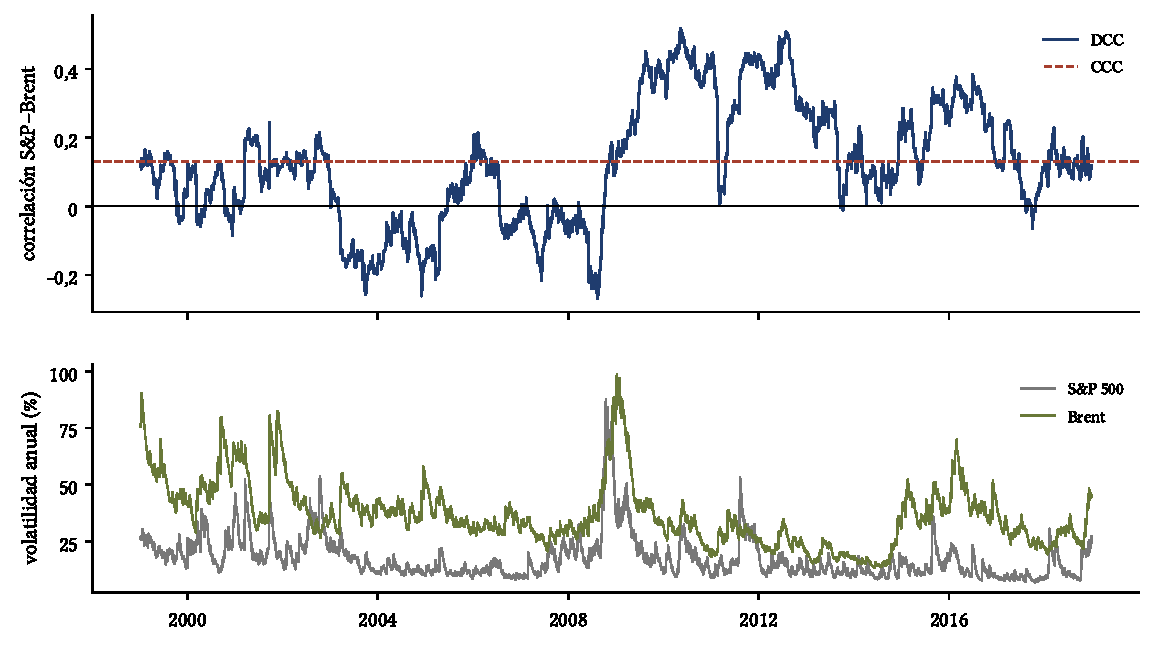
\includegraphics[width=0.92\linewidth]{graficos/cap12_ej02_dcc.pdf}
\caption{Arriba: correlación condicional DCC entre el S\&P 500 y el Brent, y la correlación constante del CCC.
Abajo: volatilidades condicionales anualizadas de la primera etapa.}
\label{fig:dcc2}
\end{figure}

\begin{conclusion}
La correlación entre el petróleo y las acciones de EE.\,UU.\ cambió de signo alrededor de 2008 y es muy
persistente. Un modelo de correlación constante habría subestimado el riesgo conjunto después de 2009.
\end{conclusion}
\end{ejresuelto}

\begin{ejresuelto}{DCC trivariado y la crisis de 2008}\label{ej:dcc3}
\enunciado Estime un DCC con las tres series y compare las correlaciones promedio en calma (enero de 2006 a
agosto de 2008), en la crisis (septiembre de 2008 a marzo de 2009) y en 2017--2018.

\solucion
\paso{Paso 1. Estimación.} $\hat a=0{,}0225$ (0,0029) y $\hat b=0{,}9732$ (0,0040); el estadístico $LR$ frente al
CCC es 788,73. El menor autovalor de las 4\,615 matrices $R_t$ es $0{,}0295$, positivo como garantiza la
Proposición~\ref{prop:dccpd}.

\paso{Paso 2. Correlaciones por período.}
\begin{center}\small
\begin{tabular}{@{}lrrr@{}}
\toprule
Período & S\&P--Nasdaq & S\&P--Brent & Nasdaq--Brent \\
\midrule
Calma 2006--2008  & 0,933 & $-0{,}053$ & $-0{,}066$ \\
Crisis 2008--2009 & 0,961 & 0,161 & 0,141 \\
2017--2018        & 0,910 & 0,103 & 0,035 \\
\bottomrule
\end{tabular}
\end{center}
Todas las correlaciones subieron en la crisis, cuando las volatilidades anuales promediaron 50\,\% en las acciones
y 71\,\% en el petróleo (Figura~\ref{fig:dcc3}).

\paso{Paso 3. Una limitación.} El DCC impone los mismos $a$ y $b$ a todos los pares. Las estimaciones cambian
al agregar el Nasdaq ($\hat a+\hat b=0{,}9957$ frente a $0{,}9974$): el modelo busca un compromiso entre la
correlación S\&P--Nasdaq, alta y estable, y la del petróleo, que cambia mucho. Hay extensiones con parámetros
por par o por grupo, a costa de más parámetros.

\codigoweb{cap12_ej03}
\salidaR{cap12_ej03_R.txt}
\lectura{cap12_ej03}

\RvsPy Para verificar que todas las $R_t$ son definidas positivas, Python calcula de una vez los autovalores
de todo el arreglo con \texttt{np.linalg.eigvalsh}. R usa \texttt{eigen} con las opciones \texttt{symmetric = TRUE} y
\texttt{only.values = TRUE} dentro de un \texttt{sapply}.

\begin{figure}[ht]
\centering
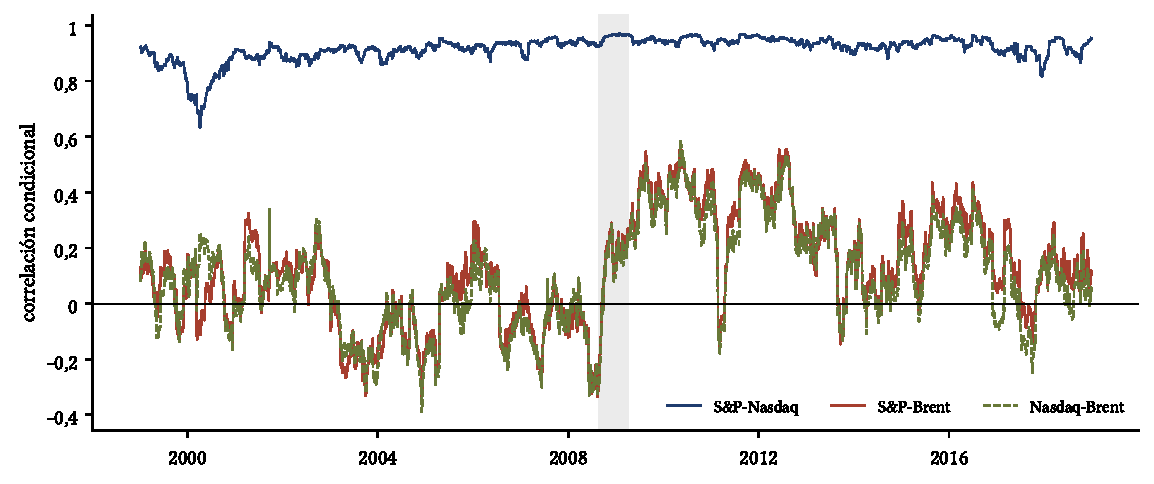
\includegraphics[width=0.92\linewidth]{graficos/cap12_ej03_dcc3.pdf}
\caption{Correlaciones condicionales del DCC trivariado. La franja gris marca la crisis de septiembre de 2008 a
marzo de 2009.}
\label{fig:dcc3}
\end{figure}

\begin{conclusion}
En la crisis de 2008 todas las correlaciones subieron a la vez. El Ejercicio~\ref{ej:contagio} pregunta si fue
contagio o un efecto mecánico de la mayor volatilidad.
\end{conclusion}
\end{ejresuelto}

\begin{ejresuelto}{Cartera de mínima varianza fuera de muestra}\label{ej:minvar}
\enunciado Con datos hasta 2009 estime los GARCH y el DCC de las tres series. Luego, con los parámetros fijos,
construya cada día de 2010--2018 la cartera de mínima varianza usando (i) la covarianza muestral constante de
1999--2009, (ii) la EWMA y (iii) el DCC-GARCH. Compare con la cartera de pesos iguales.

\solucion
\paso{Paso 1. Resultados.} Con 2\,248 días de evaluación ($\hat a=0{,}0189$ y $\hat b=0{,}9796$ en la muestra de
estimación):
\begin{center}\small
\begin{tabular}{@{}lrrrrr@{}}
\toprule
Estrategia & Volatilidad anual & Peso S\&P & Peso Nasdaq & Peso Brent & Rotación diaria \\
\midrule
Constante      & 14,56\,\% & 1,146 & $-0{,}336$ & 0,191 & 0,000 \\
EWMA           & 13,98\,\% & 1,396 & $-0{,}535$ & 0,138 & 0,206 \\
DCC            & 13,81\,\% & 1,407 & $-0{,}507$ & 0,100 & 0,128 \\
Pesos iguales  & 16,37\,\% & 0,333 & 0,333 & 0,333 & 0,000 \\
\bottomrule
\end{tabular}
\end{center}
La cartera DCC es la menos volátil. Las carteras de mínima varianza venden Nasdaq en corto para cubrir
parcialmente la exposición al S\&P 500, aprovechando su altísima correlación.

\paso{Paso 2. ¿Es significativa la diferencia?} Con la prueba de Diebold-Mariano sobre los cuadrados de los
rendimientos de cada cartera: frente a la covarianza constante, $t=4{,}33$; frente a la EWMA, $t=1{,}69$
($p=0{,}09$); frente a los pesos iguales, $t=9{,}02$. El DCC reduce significativamente el riesgo respecto de la
covarianza constante y del reparto ingenuo; su ventaja sobre la EWMA es más modesta, y además rota la cartera un
38\,\% menos ($0{,}128$ frente a $0{,}206$ de suma de cambios absolutos en los pesos por día), lo que reduce costos
de transacción.

\codigoweb{cap12_ej04}
\salidaR{cap12_ej04_R.txt}
\lectura{cap12_ej04}

\RvsPy Para no usar información futura, los GARCH y el DCC se estiman solo con 1999--2009, y después las
recursiones corren sobre toda la muestra con esos parámetros y con la $\bar Q$ de la muestra de estimación (de ahí
el argumento opcional \texttt{Qb} de \texttt{dcc\_filtro}). Los pesos usan $H_t$, que solo depende de datos hasta
$t-1$. En Python, la función de pesos se escribe en una línea con el operador \texttt{:=}.

\begin{figure}[ht]
\centering
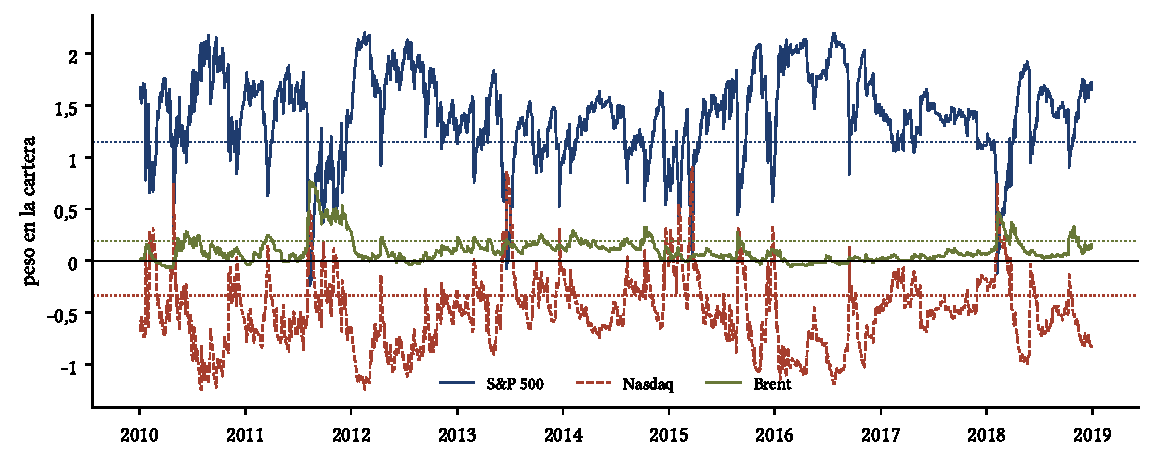
\includegraphics[width=0.92\linewidth]{graficos/cap12_ej04_pesos.pdf}
\caption{Pesos de la cartera de mínima varianza DCC en 2010--2018. Las líneas punteadas son los pesos constantes
calculados con la covarianza muestral de 1999--2009.}
\label{fig:minvar}
\end{figure}

\begin{conclusion}
Modelar la dinámica de las covarianzas tiene valor económico: la cartera DCC es un 5\,\% menos volátil que la de
covarianza constante y un 16\,\% menos que la de pesos iguales, con una rotación moderada.
\end{conclusion}
\end{ejresuelto}

\begin{ejresuelto}{¿Hubo contagio en 2008?}\label{ej:contagio}
\enunciado Compare la correlación del S\&P 500 con el Nasdaq y con el Brent en calma (enero de 2006 a agosto de
2008) y en crisis (septiembre de 2008 a marzo de 2009), antes y después de la corrección de Forbes y Rigobon,
tomando al S\&P 500 como mercado de origen. Use la transformación $z$ de Fisher para contrastar si la correlación
aumentó.

\solucion
\paso{Paso 1. El aumento de volatilidad.} La varianza diaria del S\&P 500 pasó de $1{,}0311$ a $12{,}3838$:
\begin{align*}
  \delta &= \frac{12{,}3838}{1{,}0311}-1\\
         &= 11{,}01 .
\end{align*}
La varianza se multiplicó por doce.

\paso{Paso 2. Brent.} La correlación pasó de $-0{,}113$ a $0{,}224$. Corregida:
\begin{align*}
  \rho^* &= \frac{0{,}2236}{\sqrt{1+11{,}01\,(1-0{,}2236^2)}}\\
         &= \frac{0{,}2236}{\sqrt{11{,}459}}\\
         &= \frac{0{,}2236}{3{,}385}\\
         &= 0{,}066 .
\end{align*}
Con 637 días de calma y 146 de crisis, el error estándar de la diferencia de las transformadas de Fisher es
$\sqrt{1/143+1/634}=0{,}0926$, y
\begin{align*}
  z &= \frac{\operatorname{atanh}(0{,}0661)-\operatorname{atanh}(-0{,}1131)}{0{,}0926}\\
    &= \frac{0{,}0662+0{,}1136}{0{,}0926}\\
    &= 1{,}94 .
\end{align*}
Sin la corrección, $z=3{,}68$. La corrección reduce a la mitad la evidencia de un cambio en la relación entre el
petróleo y las acciones, que queda en el límite de la significancia (valor $p$ unilateral de 0,026, bilateral de
0,052; Figura~\ref{fig:contagio}).

\paso{Paso 3. Nasdaq.} La correlación pasó de $0{,}933$ a $0{,}977$ ($z=5{,}90$), pero la corrección la reduce a
$0{,}798$ ($z=-6{,}36$), es decir, implicaría una \emph{caída} significativa. El resultado no es creíble: el S\&P 500
y el Nasdaq recibieron el mismo choque de volatilidad a la vez, y el supuesto de la
Proposición~\ref{prop:forbes} (que la varianza del componente propio de $y$ no cambie) es falso. La corrección
de Forbes y Rigobon es útil cuando el choque nace claramente en un mercado y se transmite a otro, no cuando un
factor común golpea a ambos.

\codigoweb{cap12_ej05}
\salidaR{cap12_ej05_R.txt}
\lectura{cap12_ej05}

\RvsPy La transformación de Fisher es \texttt{atanh} en R y \texttt{np.arctanh} en Python.

\begin{figure}[ht]
\centering
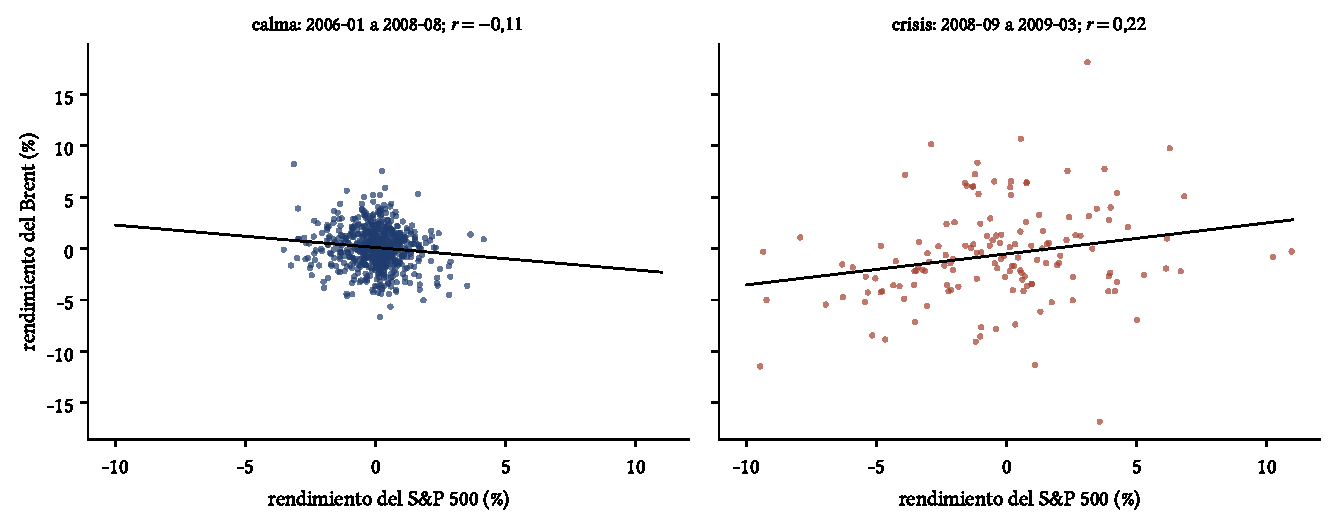
\includegraphics[width=0.92\linewidth]{graficos/cap12_ej05_contagio.pdf}
\caption{Rendimientos diarios del S\&P 500 y del Brent en calma y en crisis, con la recta de MCO. En la crisis el
rango de los rendimientos del S\&P 500 se multiplica, lo que por sí solo eleva la correlación.}
\label{fig:contagio}
\end{figure}

\begin{conclusion}
La correlación entre el petróleo y las acciones aumentó en 2008, pero una buena parte del aumento se explica por
la mayor volatilidad de las acciones. Medir contagio requiere separar el cambio en la relación del cambio en la
escala de los choques.
\end{conclusion}
\end{ejresuelto}

% ---------------------------------------------------------------------
\section{Ejercicios propuestos}
% ---------------------------------------------------------------------

\begin{enumerate}[label=\textbf{\thechapter.\arabic*},leftmargin=*,itemsep=6pt]
  \item Dos activos tienen volatilidades de 20\,\% y 30\,\% y correlación 0,3. Calcule los pesos y la volatilidad de la
  cartera de mínima varianza. \textit{Respuesta: $0{,}766$ y $0{,}234$; 18,67\,\%.}

  \item Con la Proposición~\ref{prop:forbes}, calcule la correlación medida en la crisis si $\rho=0{,}1$ y la
  varianza del mercado de origen se cuadruplica. \textit{Respuesta: $0{,}197$.}

  \item En un DCC con $a=0{,}05$, $b=0{,}93$, $\bar Q$ con unos en la diagonal y $0{,}3$ fuera de ella, y
  $Q_{t-1}=\bar Q$, calcule $\rho_t$ tras los choques $(2,2)$ y $(2,-2)$. \textit{Respuesta: $0{,}422$ y $0{,}074$.}

  \item Demuestre que, si $H_{t-1}$ es definida positiva, la EWMA multivariada produce una $H_t$ definida positiva.

  \item Demuestre que en el CCC la covarianza condicional es $h_{ij,t}=\rho_{ij}\sigma_{it}\sigma_{jt}$ y que la
  razón de cobertura de mínima varianza de $i$ con $j$ es $\rho_{ij}\sigma_{it}/\sigma_{jt}$.

  \item \emph{(Simulación.)} Simule un DCC bivariado con $a=0{,}02$, $b=0{,}97$ y GARCH(1,1) en cada serie, con
  $T=2\,000$. Estime el modelo en dos etapas 200 veces y compare la dispersión de $\hat a$ con su error estándar
  promedio. ¿Son optimistas los errores estándar de la segunda etapa?

  \item \emph{(Con datos de Yahoo Finance y el BCRP.)} Estime un DCC entre el índice S\&P/BVL Perú General, el
  precio del cobre y el tipo de cambio sol/dólar. ¿Sube la correlación entre la bolsa limeña y el cobre en los
  episodios de caída del precio de los metales?

  \item \emph{(Con datos.)} Repita el Ejercicio~\ref{ej:minvar} reestimando los parámetros cada año. ¿Cambia la
  clasificación de los modelos?
\end{enumerate}

% ---------------------------------------------------------------------
\section{Resumen de fórmulas}
% ---------------------------------------------------------------------

\begin{table}[H]
\centering\small
\begin{tabular}{@{}ll@{}}
\toprule
Concepto & Fórmula \\
\midrule
EWMA & $H_t=\lambda H_{t-1}+(1-\lambda)\boldsymbol\varepsilon_{t-1}\boldsymbol\varepsilon_{t-1}'$ \\
CCC & $H_t=D_tRD_t$,\quad $D_t=\operatorname{diag}(\sigma_{it})$ \\
DCC & $Q_t=(1-a-b)\bar Q+a\mathbf z_{t-1}\mathbf z_{t-1}'+bQ_{t-1}$;\quad $R_t=\operatorname{diag}(Q_t)^{-1/2}Q_t\operatorname{diag}(Q_t)^{-1/2}$ \\
Verosimilitud & $\ell_C=-\frac12\sum_t[\ln|R_t|+\mathbf z_t'R_t^{-1}\mathbf z_t-\mathbf z_t'\mathbf z_t]$ \\
Mínima varianza & $\mathbf w^*=H^{-1}\boldsymbol\iota/(\boldsymbol\iota'H^{-1}\boldsymbol\iota)$ \\
Forbes-Rigobon & $\rho^*=\rho_c/\sqrt{1+\delta(1-\rho_c^2)}$ \\
Fisher & $z=[\operatorname{atanh}(\rho_1)-\operatorname{atanh}(\rho_2)]/\sqrt{1/(n_1-3)+1/(n_2-3)}$ \\
\bottomrule
\end{tabular}
\caption{Fórmulas principales del Capítulo 12.}
\end{table}

\section*{Referencias}
\begin{itemize}[leftmargin=*]
  \item Bollerslev, T. (1990). Modelling the coherence in short-run nominal exchange rates: A multivariate
        generalized ARCH model. \emph{Review of Economics and Statistics}, 72(3), 498--505.
  \item Engle, R. F. (2002). Dynamic conditional correlation: A simple class of multivariate generalized
        autoregressive conditional heteroskedasticity models. \emph{Journal of Business \& Economic Statistics},
        20(3), 339--350.
  \item Engle, R. F. y Colacito, R. (2006). Testing and valuing dynamic correlations for asset allocation.
        \emph{Journal of Business \& Economic Statistics}, 24(2), 238--253.
  \item Engle, R. F. y Sheppard, K. (2001). Theoretical and empirical properties of dynamic conditional correlation
        multivariate GARCH. NBER Working Paper 8554.
  \item Forbes, K. J. y Rigobon, R. (2002). No contagion, only interdependence: Measuring stock market
        comovements. \emph{Journal of Finance}, 57(5), 2223--2261.
  \item Longin, F. y Solnik, B. (2001). Extreme correlation of international equity markets. \emph{Journal of
        Finance}, 56(2), 649--676.
\end{itemize}
